\section{Programa principal}

Antes del comienzo del ciclo BB, el proceso 0 lee la matriz y pone su testigo a verdadero. Después, este difunde al resto de procesos la matriz y el resto de procesos entra en equilibrado de carga esperando al reparto.

\begin{figure}[H]
\centering
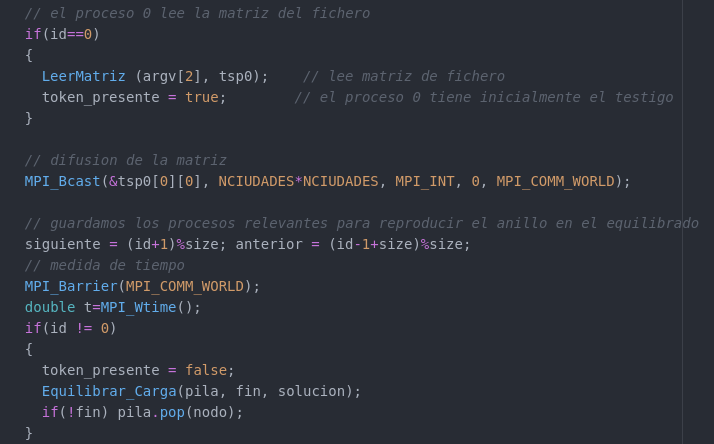
\includegraphics[width=0.8\textwidth]{imagenes/inicio.png}
\caption{Antes del ciclo BB}
\end{figure}


\begin{figure}[H]
\centering
\includegraphics[width=0.8\textwidth]{imagenes/eq_carga.png}
\caption{Equilibrado de la carga dentro del ciclo BB}
\end{figure}

\section{Equilibrado de carga}

\subsection{Comportamiento del nodo pedigüeño}

Al tener la pila vacía, manda una solicitud de carga de trabajo al siguiente proceso y realiza un sondeo de mensajes. Dependiendo del tipo de mensaje que se reciba se ejecutará una parte del código concreta.

\begin{figure}[H]
\centering
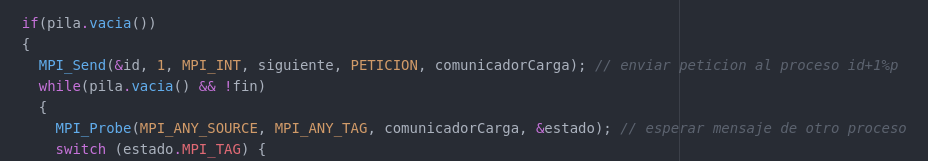
\includegraphics[width=0.8\textwidth]{imagenes/pila.png}
\caption{Entrada y sondeo de mensajes}
\end{figure}

Para la parte de peticiones de trabajo, el nodo al no tener trabajo disponible reenviará esta al siguiente nodo, pasando el testigo al proceso anterior para controlar la detección de fin.

\begin{figure}[H]
\centering
\includegraphics[width=0.8\textwidth]{imagenes/peticion_pedigueño.png}
\caption{Tratamiento de peticiones}
\end{figure}

Para poder recibir la carga de trabajo solicitada, el proceso obtiene el número de trabajos a recibir y pasa a recibirlos y almacenarlos en su pila. Pasando a ser un nodo con trabajo.

\begin{figure}[H]
\centering
\includegraphics[width=0.8\textwidth]{imagenes/nodos_pedigueño.png}
\caption{Recepción de trabajo}
\end{figure}

Con la parte de token, comprobamos si el testigo que vuelve al proceso 0 tiene el color blanco, por lo que habría llegado al fin, si no es así se sigue enviando el testigo ya que aún puede haber nodos con trabajo. Si se llegase al fin, se haría una reducción en anillo de la solución.

Si no es así, simplemente se pasa el testigo con el color correspondiente.

\begin{figure}[H]
\centering
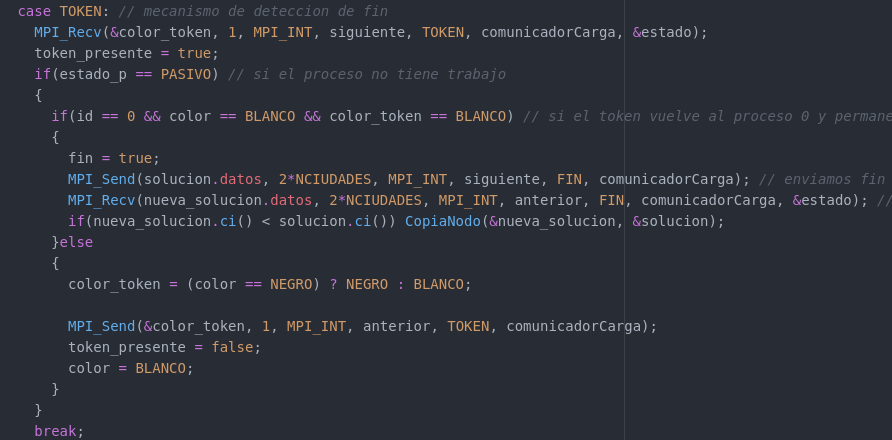
\includegraphics[width=0.8\textwidth]{imagenes/token.png}
\caption{Detección de fin}
\end{figure}

Cuando se recibe en el sondeo que se ha llegado al fin, se hace la reducción en anillo.

\begin{figure}[H]
\centering
\includegraphics[width=0.8\textwidth]{imagenes/fin_pedigueño.png}
\caption{Reducción en anillo}
\end{figure}

\subsection{Comportamiento del nodo solidario}

Cuando entra, lo primero que hace es un sondeo no bloqueante para ver si hay algún mensaje disponible, y si hay pues ejecuta la parte que corresponda.

\begin{figure}[H]
\centering
\includegraphics[width=0.8\textwidth]{imagenes/comp_solidario.png}
\caption{Sondeo no bloqueante}
\end{figure}

En la parte de petición en este caso, se obtiene la petición del proceso solicitante y se le envía la parte de trabajo correspondiente si procede, si no se reenvía la solicitud al siguiente nodo.

Si puede enviar parte de su trabajo al nodo solicitante se calcula el color del nodo para controlar la detección de fin.

\begin{figure}[H]
\centering
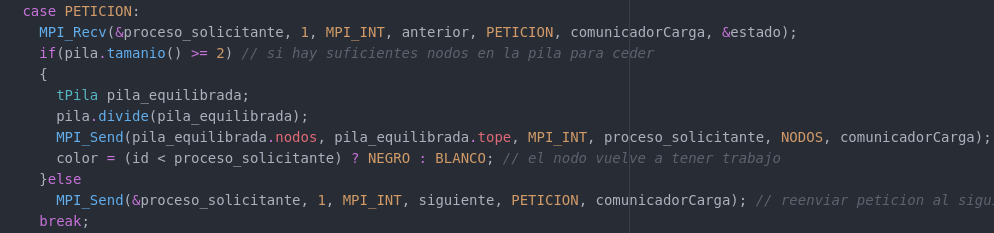
\includegraphics[width=0.8\textwidth]{imagenes/peticion_solidario.png}
\caption{Tratamiento de peticiones para el solidario}
\end{figure}

Para el token se limita a recibirlo.

\begin{figure}[H]
\centering
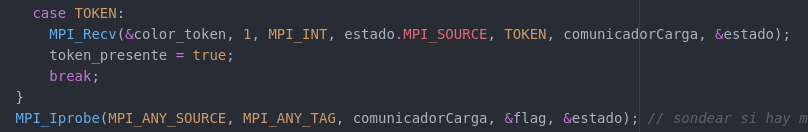
\includegraphics[width=0.8\textwidth]{imagenes/token_solidario.png}
\caption{token solidario}
\end{figure}

\section{Resultados}

\begin{figure}[H]
\centering
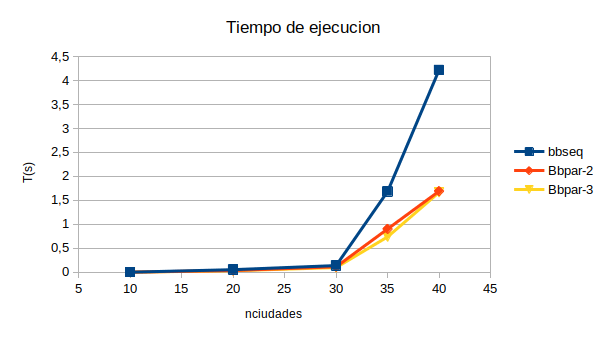
\includegraphics[width=\textwidth]{imagenes/times.png}
\caption{Tiempos de ejecución}
\end{figure}

\begin{figure}[H]
\centering
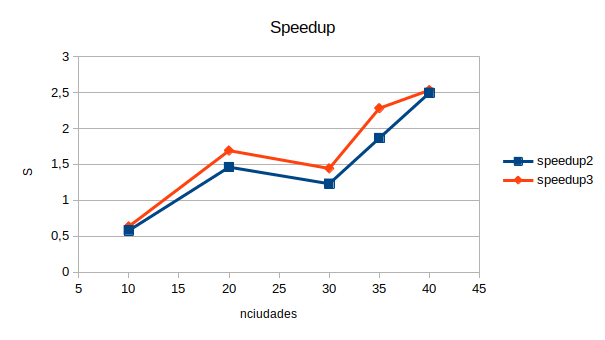
\includegraphics[width=\textwidth]{imagenes/speedup2.png}
\caption{Ganancia obtenida}
\end{figure}

\begin{table}[H]
\centering
\begin{tabular}{|l|l|}
\hline
\multicolumn{1}{|c|}{\textbf{NCIUDADES}} & \multicolumn{1}{c|}{\textbf{bbseq}} \\ \hline
10                                       & 207                                 \\ \hline
20                                       & 3755                                \\ \hline
30                                       & 6957                                \\ \hline
35                                       & 71107                               \\ \hline
40                                       & 158556                              \\ \hline
\end{tabular}
\caption{Iteraciones BB para bbseq}
\end{table}

\begin{table}[H]
\centering
\begin{tabular}{|l|l|l|}
\hline
\textbf{NCIUDADES} & \textbf{bbpar-2-p0} & \multicolumn{1}{c|}{\textbf{bbpar-2-p1}} \\ \hline
10                 & 141                 & 106                                      \\ \hline
20                 & 2388                & 2300                                     \\ \hline
30                 & 5573                & 5583                                     \\ \hline
35                 & 38208               & 38267                                    \\ \hline
40                 & 57286               & 58231                                    \\ \hline
\end{tabular}
\caption{Iteraciones BB para bbpar con np=2}
\end{table}

\begin{table}[H]
\centering
\begin{tabular}{|l|l|l|l|}
\hline
\textbf{NCIUDADES} & \textbf{Bbpar-3-p0} & \textbf{Bbpar-3-p1} & \multicolumn{1}{c|}{\textbf{Bbpar-3-p2}} \\ \hline
10                 & 111                 & 112                 & 99                                       \\ \hline
20                 & 2193                & 2100                & 2080                                     \\ \hline
30                 & 4949                & 5107                & 4804                                     \\ \hline
35                 & 32303               & 31937               & 32157                                    \\ \hline
40                 & 58104               & 56578               & 57570                                    \\ \hline
\end{tabular}
\caption{Iteraciones BB para bbpar con np=3}
\end{table}